\documentclass[12pt, a4paper]{article}

% ----- Package Imports -----
\usepackage[utf8]{inputenc}                % UTF-8 encoding
\usepackage[T1]{fontenc}                   % Output font encoding
\usepackage{mathpazo}                      % Palatino font for text and math
\usepackage{amsmath, amssymb, amsthm}      % Mathematics packages
\usepackage{graphicx}                      % Graphics inclusion
\usepackage{float}                         % Improved float handling
\usepackage{caption}                       % Custom captions
\usepackage{subcaption}                    % Subfigures
\usepackage{hyperref}                      % Hyperlinks
\usepackage[numbers]{natbib}                % Numerical citations
\usepackage{xcolor}                        % Color definitions
\usepackage[protrusion=true, expansion=true, patch=none]{microtype}                     % Improved typography
\usepackage{setspace}                      % Line spacing
\usepackage{fancyhdr}                      % Custom headers and footers
\usepackage{titlesec}                      % Custom section titles
\usepackage{booktabs}                      % Enhanced tables
\usepackage{enumitem}                      % Customized lists
\usepackage{algorithm}                     % Algorithms
\usepackage{algpseudocode}                 % Pseudocode
\usepackage{mathtools}                     % Enhanced math features
\usepackage{geometry}                      % Page layout
\usepackage{doi}                           % DOI links in bibliography
\usepackage{tikz}                          % TikZ diagrams
\usepackage{listofitems}
\usepackage[outline]{contour} % glow around text
\usetikzlibrary{positioning, shapes, arrows.meta, calc, positioning, shapes.geometric}
\contourlength{1.4pt}

% ----- Figures configuration -----
\graphicspath{{figures/}}                  % Path to figures
\captionsetup{font=small, labelfont=bf}     % Caption settings
\captionsetup[sub]{font=small}             % Subcaption settings

% ----- Page Layout -----
\geometry{
    a4paper,
    left=1in,
    right=1in,
    top=1in,
    bottom=1in,
}

% ----- Typography and Spacing -----
\microtypesetup{protrusion=true, expansion=true}  % Microtype settings
\setstretch{1.5}                                 % Line spacing set to 1.5

% ----- Custom Colors -----
\definecolor{accentred}{RGB}{204, 0, 0}
\definecolor{accentblue}{RGB}{0, 102, 204}
\definecolor{accentgreen}{RGB}{0, 153, 0}
\definecolor{lightgray}{RGB}{240, 240, 240}


% ----- Hyperlink Configuration -----
\hypersetup{
    colorlinks=true,
    linkcolor=accentblue,       % Internal links (sections, etc.)
    citecolor=accentgreen,      % Citation links
    urlcolor=accentred,         % External URLs
    linktoc=all,                % Links include both text and page number in TOC
    pdfauthor={Your Name},
    pdftitle={Fluid-Structure Interaction Analysis of Pulsatile Flow in Arterial Aneurysms with Physics-Informed Neural Networks and Computational Fluid Dynamics},
    pdfsubject={Research Paper},
}


% ----- Header and Footer Configuration -----
\pagestyle{fancy}
\setlength{\headheight}{14.49998pt}
\addtolength{\topmargin}{-2.49998pt}
\fancyhf{}  % Clear all header and footer fields
\fancyhead[L]{\nouppercase{\leftmark}}  % Left header: section title
\fancyhead[R]{\thepage}                 % Right header: page number
\renewcommand{\headrulewidth}{0.5pt}    % Header rule
\renewcommand{\footrulewidth}{0pt}      % No footer rule

% ----- Section Title Configuration -----
\titleformat{\section}
  {\normalfont\Large\bfseries\color{accentblue}}{\thesection}{1em}{}

\titleformat{\subsection}
  {\normalfont\large\bfseries\color{accentgreen}}{\thesubsection}{1em}{}

\titleformat{\subsubsection}
  {\normalfont\normalsize\bfseries\color{accentgreen}}{\thesubsubsection}{1em}{}

% ----- Title and Author -----
\title{
    \vspace{-2cm} % Adjust vertical spacing as needed
    \large \textbf{Fluid-Structure Interaction Analysis of Pulsatile Flow in Arterial Aneurysms with Physics-Informed Neural Networks and Computational Fluid Dynamics}\\
}

\author{
    Michael Ajao-Olarinoye\textsuperscript{1} \\
    \textsuperscript{1}Center for computational science and Mathematical modelling \\
    \texttt{olarinoyem@coventry.ac.uk}
}

\date{}

\begin{document}

\maketitle



\section{Physics-Informed Neural Networks}
\label{sec:PINNs}

% \subsection{overview}
% \label{sec:PINN_Overview}

High-fidelity Computational Fluid Dynamics (CFD) simulations, as outlined in Section~2.4, offer precise insights into arterial hemodynamics and are central to modeling fluid dynamics in complex vascular geometries. However, these simulations can be both computationally expensive and time-consuming, especially when dealing with patient-specific anatomies or conducting numerous parameter sweeps. Such challenges are further compounded by the need for significant domain expertise to refine meshes, tune solvers, and interpret results.

Physics-Informed Neural Networks (PINNs), first introduced by \citet{raissi2019physics}, have emerged as a powerful alternative that combines the strengths of traditional deep learning with established physics-based modeling. Rather than relying exclusively on data-driven learning, PINNs integrate the governing partial differential equations (PDEs) in this case, the continuity and momentum conservation equations (Section~2.2) directly into the network's loss function. This approach ensures that the neural network is ``informed'' by the physical laws of fluid motion, guiding it toward realistic flow solutions even when labeled data are sparse or imperfectly measured.

By integrating PDE residuals and boundary conditions into the training process, PINNs inherently enforce the fundamental laws of fluid dynamics, yielding physically consistent solutions even with limited labeled data. This physics-based integration minimizes overfitting and eliminates the need for conventional mesh discretization, enabling the network to be evaluated at arbitrary spatial and temporal resolutions, as a result, they can effectively complement or even partially replace traditional CFD simulations. Moreover, the outputs of PINNs can be used to generate high-resolution flow fields predictions that exceed the original CFD. Consequently, once trained, PINNs provide rapid inference and are highly adaptable to new boundary conditions or geometrical changes with minimal retraining, making them an efficient, mesh-free alternative to traditional CFD simulations \citep{jagtap2020extended}.

Furthermore, the mesh-free framework of PINNs eliminates the need for domain discretization, thereby simplifying simulation workflows and reducing computational overhead. This attribute is particularly beneficial for complex geometries like arterial aneurysms, where conventional CFD methods often face challenges during mesh generation \citep{zhang2024meshless, bhargava2024enhancing}. Techniques like adaptive weighted loss functions further improve prediction accuracy and generalization capabilities, making PINNs a versatile tool for a wide range of fluid dynamics applications \citep{liu2024variable}.

Although PINNs provide numerous benefits, ensuring robust and accurate simulations across various physiological conditions remains a challenge. Incorporating clinical data and further refining the neural network architectures could significantly broaden the utility of PINNs in real-world cardiovascular diagnostics and treatment planning.

In this study, we combine PINNs with traditional CFD data to estimate core hemodynamic variables such as pressure, velocity components, and wall shear stress (WSS) across healthy and Marfan Syndrome aortic geometries presented in (Section~2.1). This unified approach enables direct comparisons of velocity patterns, shear forces, and other critical flow indicators between non-pathological and aneurysmal models, providing valuable information for understanding the progression of vascular disease. The following sections detail the formulation, architecture, and training strategy of the PINNs used in this study.

\subsection{Formulation of Physics-Informed Neural Networks}
\label{sec:PINN_Formulation}

Modeling pulsatile flow in arterial segments necessitates the enforcement of both the continuity and momentum conservation equations to capture the essential hemodynamic effects. In this work, blood flow is modeled using the Reynolds-averaged Navier–Stokes (RANS) equations (see Sections~2.2 and 2.3), which describe the flow behavior in the aortic geometries. Let \(\mathbf{u} = (u,v,w)\) denote the velocity field, \(p\) the pressure, \(\rho\) the fluid density, and \(\mu\) the dynamic viscosity. The continuity and momentum conservation equations are combined to form the Navier–Stokes system, which governs the evolution of the velocity field and pressure in response to external forces and viscous effects.

The boundary conditions employed in the simulations include a no-slip condition on the arterial walls \((\mathbf{u} = \mathbf{0} \text{ on } \partial\Omega_{\mathrm{wall}})\), zero relative pressure at the outlet, and a pulsatile inlet velocity prescribed on the inlet boundary \((\partial\Omega_{\mathrm{inlet}})\) as detailed in Equation~(2.1) (Section~2.3). These boundary and inlet constraints are incorporated into the PINNs through penalty terms in the loss function, ensuring that the network’s predictions adhere to the specified physical conditions. In addition, the temporal dependence is explicitly modeled to reflect the transient nature of blood flow.

Within the PINN framework, the neural network approximates the functions
\[
u(x,y,z,t),\quad v(x,y,z,t),\quad w(x,y,z,t),\quad p(x,y,z,t),
\]
as well as the corresponding wall shear stress (WSS) components
\[
\tau_x(x,y,z,t),\quad \tau_y(x,y,z,t),\quad \tau_z(x,y,z,t).
\]
Collectively, these functions capture the spatiotemporal evolution of blood flow and the shear forces acting on the vessel walls.

Let \(F(\cdot)\) denote the non-linear operator corresponding to the Navier–Stokes system of equations as defined in Equation~(3.1). The physics residual loss is then defined as
\begin{equation}
L_{\mathrm{physics}} = \Bigl\|F(\mathbf{u}, p)\Bigr\|_2,
\end{equation}
where \(\|\cdot\|_2\) represents the Euclidean norm. Minimization of this loss drives the PINN to approximate velocity and pressure fields that satisfy the Navier–Stokes equations, thereby capturing the fundamental flow dynamics even in regions with sparse or missing data.

Furthermore, the loss function includes additional terms to enforce the boundary conditions. Specifically, the penalty for the no-slip condition and the prescribed inlet velocity are given by
\begin{equation}
L_{\mathrm{boundary}} = \Bigl\|\mathbf{u}\big|_{\partial\Omega_{\mathrm{wall}}} - \mathbf{0}\Bigr\|_2,\quad
L_{\mathrm{inlet}} = \Bigl\|\mathbf{u}\big|_{\partial\Omega_{\mathrm{inlet}}} - \mathbf{u}_{\mathrm{inlet}}(t)\Bigr\|_2,
\end{equation}
where \(\mathbf{u}_{\mathrm{inlet}}(t)\) is the time-varying inlet velocity profile. When available, CFD reference data for pressure, velocity, and WSS are incorporated into the training through a data loss term. Let \(\mathbf{u}_{\mathrm{NN}}\) and \(p_{\mathrm{NN}}\) denote the predictions of the PINN, while \(\mathbf{u}_{\mathrm{CFD}}\) and \(p_{\mathrm{CFD}}\) denote the corresponding CFD reference data. The data loss term is defined as
\begin{equation}
L_{\mathrm{data}} = \Bigl\|\mathbf{u}_{\mathrm{NN}} - \mathbf{u}_{\mathrm{CFD}}\Bigr\|_2 + \Bigl\|p_{\mathrm{NN}} - p_{\mathrm{CFD}}\Bigr\|_2 + \Bigl\|\boldsymbol{\tau}_{\mathrm{NN}} - \boldsymbol{\tau}_{\mathrm{CFD}}\Bigr\|_2.
\end{equation}

The total loss function is then formulated as
\begin{equation}
L_{total} = \lambda_{\mathrm{physics}}\,L_{\mathrm{physics}} + \lambda_{\mathrm{boundary}}\,L_{\mathrm{boundary}} + \lambda_{\mathrm{inlet}}\,L_{\mathrm{inlet}} + \lambda_{\mathrm{data}}\,L_{\mathrm{data}},
\label{eq:total_loss}
\end{equation}
where \(\lambda_{\mathrm{physics}}, \lambda_{\mathrm{boundary}}, \lambda_{\mathrm{inlet}}, \lambda_{\mathrm{data}}\) are self-adaptive weighting coefficients~\citep{mcclenny2020self}. These coefficients are optimized during training to automatically balance the importance of each loss component, ensuring that the PINN faithfully respects the fundamental fluid dynamics as well as the available CFD data. The training workflow for the PINNs, which encompasses the forward pass, loss computation, and weight updates via backpropagation, is illustrated in Figure~\ref{fig:training_workflow}.



% \subsection{Formulation of Physics-Informed Neural Networks}
% \label{sec:PINN_Formulation}

% Modeling pulsatile flow in arterial segments requires enforcing both the continuity and momentum conservation equations to capture the essential hemodynamic effects. In our work, the blood flow is modeled based on the Reynolds-averaged Navier–Stokes (RANS) equations (see Sections~2.2 and 2.3), which describe the flow in the aortic geometries. Let \(\mathbf{u} = (u,v,w)\) denote the velocity field, \(p\) the pressure, \(\rho\) the fluid density, and \(\mu\) the dynamic viscosity. The continuity and momentum conservation equations are combined to form the Navier–Stokes system, which describes the evolution of the velocity field and pressure in response to external forces and viscous effects. 

% The boundary conditions involve a no-slip condition on the arterial walls \((\mathbf{u}=\mathbf{0} \text{ on } \partial\Omega_{\text{wall}})\), zero relative pressure at the outlet, and a pulsatile inlet velocity on the inlet boundary as \(\partial\Omega_{\text{inlet}}\) detailed in Equation~2.1 (Section~2.3) respectively. These boundary and inlet constraints are incorporated into the PINNs through penalty terms in the loss function, thereby enforcing consistency between the network’s predictions and the specified physical conditions. Temporal dependence is explicitly modelled to reflect the transient nature of blood flow.

% Within the PINN framework, neural networks approximate the velocity field \(\mathbf{u}\), pressure \(p\), and wall shear stress (WSS) components \(\tau_x, \tau_y, \tau_z\) as functions of the spatial coordinates \((x,y,z)\) and time \(t\). The network architecture is trained to minimise the physics residual loss, which quantifies the deviation of the predicted solutions from the Navier--Stokes and continuity equations. 

% \[
%     u(x,y,z,t),\quad v(x,y,z,t),\quad w(x,y,z,t),\quad p(x,y,z,t),
% \]
% as well as the three wall shear stress (WSS) components 
% \[
%     \tau_x(x,y,z,t),\quad \tau_y(x,y,z,t),\quad \tau_z(x,y,z,t).
% \]
% Together, these variables capture the spatiotemporal evolution of blood flow and the shear forces acting on the vessel walls.

% Let \(F(\cdot)\) represent the non-linear operator corresponding to the Navier--Stokes system of equations as defined in Equation~(3.1). The physics residual loss is defined as the Euclidean norm of the residual terms, which ensures that the network learns solutions consistent with the governing equations even in regions with sparse or missing data. The physics loss term is given by:

% \begin{equation}
% L_{\mathrm{physics}} = \bigl\|F(\mathbf{u}, p)\bigr\|_2,
% \end{equation}

% where \(\|\cdot\|_2\) denotes the Euclidean norm. By minimising this residual, the PINN learns to approximate the velocity and pressure fields that satisfy the Navier--Stokes equations, thereby capturing the essential flow dynamics within the arterial geometries.

% Arterial boundaries impose \(\mathbf{u}=\mathbf{0}\) at the vessel walls and zero pressure at the outlet, while a prescribed pulsatile velocity profile is enforced at the inlet:
% \begin{equation}
% L_{\mathrm{boundary}} = \|\mathbf{u}\big|_{\partial\Omega_{\text{wall}}} - \mathbf{0}\|_2, 
% \quad
% L_{\mathrm{inlet}} = \|\mathbf{u}\big|_{\Gamma_{\mathrm{inlet}}} - \mathbf{u}_{\mathrm{inlet}}(t)\|_2.
% \end{equation}
% where \(\partial\Omega_{\mathrm{wall}}\) and \(\partial\Omega_{\mathrm{inlet}}\) denote the wall and inlet boundaries, respectively, and \(\mathbf{u}_{\mathrm{inlet}}(t)\) is the prescribed pulsatile inlet velocity profile (Section~2.3). These terms penalise any deviation of the network’s predictions from the specified boundary conditions, thus reinforcing physically realistic flow fields at the walls and inflow region.

% When available, data for pressure, velocity and wss were integrated into the loss function. Let \(\mathbf{u}_{\mathrm{NN}}\) and \(p_{\mathrm{NN}}\) denote the PINN’s predicted velocity and pressure, while \(\mathbf{u}_{\mathrm{CFD}}\) and \(p_{\mathrm{CFD}}\) are the corresponding CFD reference fields. Here, the subscripts “NN” and “CFD” distinguish between the network’s predictions and the CFD reference ground truth data. The data loss term is defined as:

% \begin{equation}
% L_{\mathrm{data}} = 
% \|\mathbf{u}_{\mathrm{NN}} - \mathbf{u}_{\mathrm{CFD}}\|_2 
% + \|p_{\mathrm{NN}} - p_{\mathrm{CFD}}\|_2
% + \|\tau_{\mathrm{NN}} - \tau_{\mathrm{CFD}}\|_2.
% \end{equation}

% The total loss combines physics, boundary, inlet, and data objectives:
% \begin{equation}
% L_{total} = 
% \lambda_{\mathrm{physics}}\,L_{\mathrm{physics}}
% + \lambda_{\mathrm{boundary}}\,L_{\mathrm{boundary}}
% + \lambda_{\mathrm{inlet}}\,L_{\mathrm{inlet}}
% + \lambda_{\mathrm{data}}\,L_{\mathrm{data}},
% \label{eq:total_loss}
% \end{equation}

% where \(\lambda_{\mathrm{physics}}, \lambda_{\mathrm{boundary}}, \lambda_{\mathrm{inlet}}, \lambda_{\mathrm{data}}\) are self-adaptive weighting coefficients~\citep{mcclenny2020self}. These learnable parameters automatically balance the importance of each loss component during training, ensuring that the PINN respects both the fundamental equations of fluid motion and the given available CFD data. The self-adaptive weighting mechanism is explained futher in Section~\ref{sec:self_adaptive_weighting}. The training workflow for the PINNs is illustrated in Figure~\ref{fig:training_workflow}, highlighting the forward pass, loss computation, and weight updates during the training process.

\subsection{Neural Network Architecture}
\label{sec:PINN_Architecture_Training}

The neural network architecture plays a crucial role in the performance and generalisation capabilities of PINNs. In this study, We train separate PINNs for pressure $p$, velocity components $(u, v, w)$, and the three WSS components $(\tau_x, \tau_y, \tau_z)$, all time dependant $(t)$. Each network is a feed-forward, fully connected architecture with $L=10$ hidden layers and $N=64$ neurons per layer. The Swish activation function \citep{ramachandran2017searching} is employed to promote smooth gradients. batch normalization is applied to each layer to stabilize training, and all weights are initialized using Kaiming normal \citep{he2015delving} to ensure stable gradient flow.

The Swish activation function~\cite{ramachandran2017searching} is defined as:
\begin{equation}
\mathrm{Swish}(x) = x \,\sigma(\beta x),
\end{equation}
where $\beta$ is a learnable parameter and $\sigma(\cdot)$ is the sigmoid function. This choice often yields faster convergence compared to ReLU or other activations. The network architecture is visualized in Figure~\ref{fig:nn_architecture}, illustrating the flow of spatial-temporal coordinates $(x, y, z, t)$ through the hidden layers to predict the pressure, velocity, and WSS components.

\begin{figure}[htbp]
    \centering
    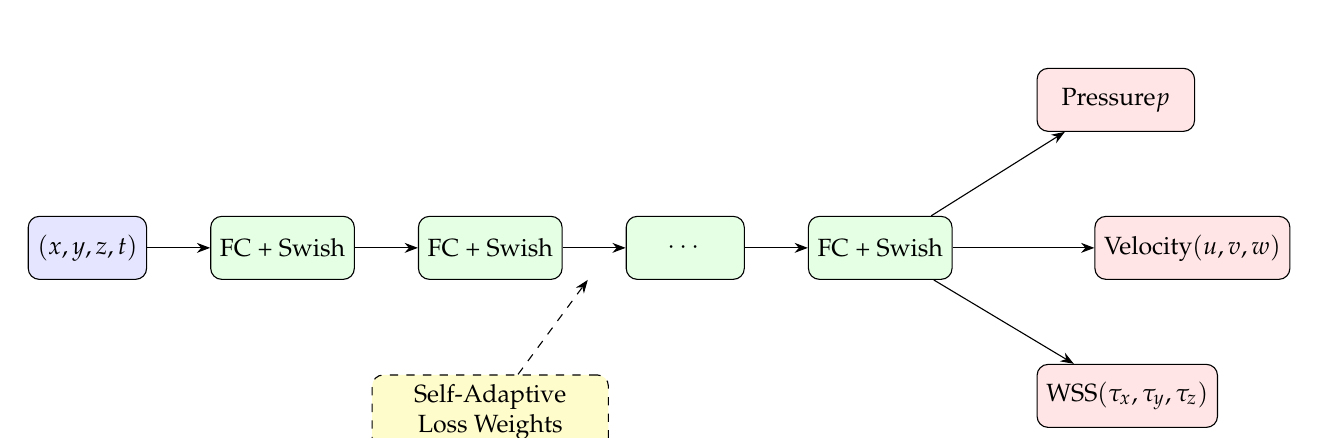
\begin{tikzpicture}[node distance=0.8cm, auto, >=Stealth,
        every node/.style={font=\small}]
      % Input node
      \node[draw, rectangle, rounded corners, minimum width=1.5cm, minimum height=0.8cm, fill=blue!10] (input) {$(x,y,z,t)$};
      
      % Hidden layers
      \node[draw, rectangle, rounded corners, right=of input, minimum width=1.5cm, minimum height=0.8cm, fill=green!10] (h1) {FC + Swish};
      \draw[->] (input) -- (h1);
      
      \node[draw, rectangle, rounded corners, right=of h1, minimum width=1.5cm, minimum height=0.8cm, fill=green!10] (h2) {FC + Swish};
      \draw[->] (h1) -- (h2);
      
      \node[draw, rectangle, rounded corners, right=of h2, minimum width=1.5cm, minimum height=0.8cm, fill=green!10] (dots) {$\cdots$};
      \draw[->] (h2) -- (dots);
      
      \node[draw, rectangle, rounded corners, right=of dots, minimum width=1.5cm, minimum height=0.8cm, fill=green!10] (hFinal) {FC + Swish};
      \draw[->] (dots) -- (hFinal);
      
      % Output branches
      \node[draw, rectangle, rounded corners, above right=of hFinal, xshift=0.5cm, yshift=0.5cm, minimum width=2cm, minimum height=0.8cm, fill=red!10] (pOut) {Pressure\\$p$};
      \node[draw, rectangle, rounded corners, right=of hFinal, xshift=1.0cm, minimum width=2cm, minimum height=0.8cm, fill=red!10] (vOut) {Velocity\\$(u,v,w)$};
      \node[draw, rectangle, rounded corners, below right=of hFinal, xshift=0.5cm, yshift=-0.5cm, minimum width=2cm, minimum height=0.8cm, fill=red!10] (wOut) {WSS\\$(\tau_x,\tau_y,\tau_z)$};
      
      \draw[->] (hFinal) -- (pOut);
      \draw[->] (hFinal) -- (vOut);
      \draw[->] (hFinal) -- (wOut);
      
      % Self-adaptive weights block (dashed) below hidden layers
      \node[draw, rectangle, dashed, rounded corners, below=1.2cm of h2, minimum width=3cm, minimum height=0.8cm, fill=yellow!20, align=center] (weights) {Self-Adaptive\\Loss Weights};
      \draw[->, dashed] (weights) -- ($(h2.south)!0.5!(dots.south)$);
    \end{tikzpicture}
    \caption{Architecture for predicting pressure, velocity, and WSS from spatiotemporal inputs \((x,y,z,t)\) via fully connected layers with Swish activations. The network branches into three outputs and includes self-adaptive loss weights.}
    \label{fig:nn_architecture}
\end{figure}


\subsubsection{Self-Adaptive Loss Weighting Scheme}
\label{sec:self_adaptive_weighting}

The self-adaptive loss weighting scheme is a key component of the PINN training process, enabling the network to dynamically adjust the relative importance of different loss components based on their contributions to the total loss. This mechanism prevents any single loss term from dominating, thereby ensuring that the network effectively balances the physics residuals, boundary conditions, inlet constraints, and supervised data.

Balancing multiple loss components is particularly challenging in multi-physics scenarios, where various physical phenomena and boundary conditions must be simultaneously satisfied \citep{mcclenny2020self}. In our study, the primary loss components include the physics residuals derived from the governing PDEs, the boundary conditions, the inlet conditions, and the supervised data from CFD simulations. Improper weighting of these components can lead to suboptimal training outcomes, such as overfitting or failure to capture the underlying physical laws.

To address this challenge, we implement a self-adaptive loss weighting scheme inspired by \citet{mcclenny2020self}. Specifically, we introduce learnable parameters \(\log \lambda_i\) for each loss component \(i \in \{\mathrm{phys}, \mathrm{bound}, \mathrm{inlet}, \mathrm{data}\}\). These parameters are optimized jointly with the network weights during training, and the corresponding weights are defined as

\begin{equation}
    \lambda_i = \exp(\log \lambda_i),
    \label{eq:lambda_definition}
\end{equation}

which ensures that each \(\lambda_i\) remains positive throughout training. By automatically adjusting \(\log \lambda_i\), the network dynamically balances the contributions of each loss component based on the training dynamics, eliminating the need for manual tuning of hyperparameters and facilitating a more stable and efficient convergence \citep{wang2022and}. The self-adaptive weighting scheme is implemented as part of the total loss function in Equation~\eqref{eq:total_loss}, where the loss components are weighted by the corresponding \(\lambda_i\) coefficients. The self-adaptive weighting mechanism is summarized in Algorithm~\ref{alg:self_adaptive_weighting}. 


\begin{algorithm}[htbp]
    \caption{Self-Adaptive Loss Weighting in PINNs}
    \label{alg:self_adaptive_weighting}
    \begin{algorithmic}[1]
    \Require Initial network weights $\theta$, initial $\log \lambda_i$, learning rates for $\theta$ and $\log \lambda_i$
    \Ensure Trained network weights $\theta^*$ and optimized $\lambda_i^*$
    
    \While{not converged}
        \State Sample mini-batch of training points
        \State Forward pass to compute predictions $\mathbf{u}_{\mathrm{NN}}$, $p_{\mathrm{NN}}$, $\boldsymbol{\tau}_{\mathrm{NN}}$
        
        \State Compute individual loss components:
            \State \quad $\mathcal{L}_{\mathrm{phys}} = \|F(\mathbf{u}_{\mathrm{NN}}, p_{\mathrm{NN}})\|_2^2$
            \State \quad $\mathcal{L}_{\mathrm{bound}} = \|\mathbf{u}_{\mathrm{NN}}|_{\partial\Omega_{\mathrm{wall}}} - \mathbf{0}\|_2^2$
            \State \quad $\mathcal{L}_{\mathrm{inlet}} = \|\mathbf{u}_{\mathrm{NN}}|_{\Gamma_{\mathrm{inlet}}} - \mathbf{u}_{\mathrm{inlet}}(t)\|_2^2$
            \State \quad $\mathcal{L}_{\mathrm{data}} = \|\mathbf{u}_{\mathrm{NN}} - \mathbf{u}_{\mathrm{CFD}}\|_2^2 + \|p_{\mathrm{NN}} - p_{\mathrm{CFD}}\|_2^2 + \|\boldsymbol{\tau}_{\mathrm{NN}} - \boldsymbol{\tau}_{\mathrm{CFD}}\|_2^2$
        
        \State \quad $\mathcal{L}_{\mathrm{total}} = \lambda_{\mathrm{phys}} \mathcal{L}_{\mathrm{phys}} + \lambda_{\mathrm{bound}} \mathcal{L}_{\mathrm{bound}} + \lambda_{\mathrm{inlet}} \mathcal{L}_{\mathrm{inlet}} + \lambda_{\mathrm{data}} \mathcal{L}_{\mathrm{data}}$
        
        \State Backpropagate the total loss to compute gradients for $\theta$ and $\log \lambda_i$
        
        \State Update network weights $\theta \gets \theta - \eta_{\theta} \nabla_{\theta} \mathcal{L}$
        \State Update log-weights $\log \lambda_i \gets \log \lambda_i - \eta_{\lambda} \nabla_{\log \lambda_i} \mathcal{L}$
        
        \State StepLR scheduler updates learning rates $\eta_{\theta}$ and $\eta_{\lambda}$ every $N$ epochs
    \EndWhile
    
    \State \textbf{Return} $\theta^*$, $\lambda_i^*$
    \end{algorithmic}
\end{algorithm}

The self-adaptive loss weighting algorithm is summarized in Algorithm~\ref{alg:self_adaptive_weighting}. During training, the network weights \(\theta\) and the log-weights \(\log \lambda_i\) are updated simultaneously using stochastic gradient descent. The loss components are computed for each mini-batch, and the total loss is evaluated based on the current predictions and the CFD reference data. The gradients of the total loss with respect to the network weights and log-weights are then backpropagated to update the parameters. A StepLR scheduler is employed to adjust the learning rates for the network weights and log-weights every \(N\) epochs, ensuring stable convergence and preventing oscillations during training. The self-adaptive weighting mechanism enables the network to effectively balance the physics residuals, boundary conditions, inlet constraints, and supervised data, leading to robust and accurate predictions of arterial flow dynamics.

\begin{figure}[htbp]
    \centering
    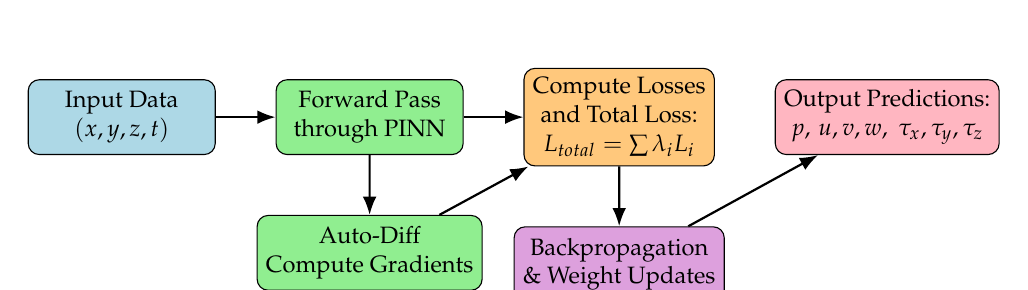
\begin{tikzpicture}[node distance=0.8cm, auto, >=Latex, every node/.style={font=\small}, scale=0.95, transform shape]
    % Define a block style
    \tikzset{
        block/.style={draw, rectangle, rounded corners, align=center, minimum width=2.5cm, minimum height=1cm},
    }
    % Define colors for different blocks
    \definecolor{inputblue}{RGB}{173,216,230}
    \definecolor{processgreen}{RGB}{144,238,144}
    \definecolor{lossorange}{RGB}{255,200,124}
    \definecolor{updatepurple}{RGB}{221,160,221}
    \definecolor{outputred}{RGB}{255,182,193}
    
    % Nodes
    \node[block, fill=inputblue] (data) {Input Data\\\((x,y,z,t)\)};
    \node[block, fill=processgreen, right=of data] (forward) {Forward Pass\\through PINN};
    \node[block, fill=lossorange, right=of forward] (loss) {Compute Losses\\and Total Loss:\\\(L_{total}=\sum \lambda_i L_i\)};
    \node[block, fill=updatepurple, below=of loss] (backprop) {Backpropagation\\\& Weight Updates};
    \node[block, fill=outputred, right=of loss] (predict) {Output Predictions:\\\(p,\,u,v,w,\;\tau_x,\tau_y,\tau_z\)};
    \node[block, fill=processgreen, below=of forward] (grad) {Auto-Diff\\Compute Gradients};
    
    % Arrows connecting the nodes
    \draw[->, thick] (data) -- (forward);
    \draw[->, thick] (forward) -- (grad);
    \draw[->, thick] (forward) -- (loss);
    \draw[->, thick] (grad) -- (loss);
    \draw[->, thick] (loss) -- (backprop);
    \draw[->, thick] (backprop) -- (predict);
    
    \end{tikzpicture}
    \caption{PINN training workflow: input \((x,y,z,t)\) undergoes forward propagation and backpropagation to update the network and yield pressure, velocity, and WSS predictions.}
    \label{fig:training_workflow}
\end{figure}


% \subsection{Data Processing and Experimental Setup}
% \label{sec:data_processing}

% The experimental data were obtained from CFD simulations of both healthy and aneurysmal aortic geometries, with measurements captured during both systolic and diastolic phases. Each dataset includes spatial coordinates (X, Y, Z), time points, pressure values, velocity components (u, v, w), and wall shear stress (WSS) components. Prior to model training, the raw data underwent a systematic preprocessing procedure. First, the data were cleaned by removing incomplete records and verifying the physical consistency of the measurements, resulting in a final dataset (e.g, 0021 dystolic aneurysm) comprising approximately 11,005 spatial points per time step in the dataset. Subsequently, all input features and target variables were normalized using Min–Max scaling, ensuring stable training across the network. Specifically, spatial coordinates were scaled to the range \([-1,1]\), over the cardiac cycle, and each of the physical variables (pressure, velocity, and WSS components) was scaled independently. To enforce the no-slip condition at the vessel walls, boundary points were identified using a velocity magnitude threshold (\(|u|,\, |v|,\, |w| < 10^{-5}\)). The processed data were then organized by case healthy cases (0024 and 0142) and aneurysmal cases (0021, 0022, 0023, and 0025) with uniform temporal sampling across the cardiac cycle. Finally, quality control measures were applied, including physical consistency checks on velocity and pressure fields, validation of WSS components against analytical solutions, verification of mass conservation at the inlet and outlet boundaries, and confirmation of temporal continuity across cardiac cycles. 


% \subsection{Training of the PINNs for Pulsatile Flow Simulations}
% \label{sec:training_PINNs}

% The PINN framework was implemented in \texttt{Python} using the PyTorch library \citep{paszke2019pytorch}, which leverages automatic differentiation for efficient computation of PDE residuals. All codes and numerical experiments for the PINN-based aneurysm flow analyses were developed using PyTorch, with the self-adaptive weighting and physics-based PDE residuals integrated into the backpropagation routine. The detailed hyperparameters and training protocol, as described below, ensure reproducibility and transparency.

% Input spatiotemporal data points \((x_j, y_j, z_j, t_j)\) were randomly sampled from the aortic geometries over the cardiac cycle and normalized via Min–Max scaling. The PINNs were trained using the AdamW optimizer \citep{loshchilov2017decoupled} with an initial learning rate of \(1\times10^{-4}\), momentum parameters \(\beta=(0.9,0.999)\), and a weight decay of \(1\times10^{-4}\). A StepLR scheduler reduced the learning rate by a factor of \(\gamma=0.9\) every 200 epochs to facilitate finer convergence.

% Training was performed using mixed-precision arithmetic via \texttt{torch.cuda.amp} \citep{micikevicius2017mixed} to enhance computational efficiency and reduce memory consumption without compromising accuracy. The training process was iterated for up to 1000 epochs, with early stopping implemented if the validation loss did not decrease for 5 consecutive epochs. Gradient clipping was applied with a maximum norm of 1.0 to prevent exploding gradients. The entire training was executed on a high-performance computing cluster equipped with NVIDIA RTX 8000 GPUs, which enabled efficient parallel processing and rapid convergence. The overall training workflow, illustrated in Figure~\ref{fig:training_workflow}, encompasses the forward pass, loss computation (including physics, boundary, inlet, and data losses combined as \(L_{total}=\sum \lambda_i L_i\)), and subsequent backpropagation and weight updates.



\subsection{Data Processing and Experimental Setup}
\label{sec:data_processing}

The experimental data were derived from CFD simulations of both healthy and aneurysmal aortic geometries, with measurements acquired during the systolic and diastolic phases. Each dataset comprises spatial coordinates (X, Y, Z), time points, pressure values, velocity components (u, v, w), and wall shear stress (WSS) components. Prior to model training, the raw data underwent a comprehensive preprocessing pipeline. Initially, the data were cleaned by removing incomplete records and verifying the physical consistency of the measurements, resulting in, for example, the 0021 diastolic aneurysm dataset containing approximately 11,005 spatial points per time step. Subsequently, all input features and target variables were normalized via Min–Max scaling; spatial coordinates were scaled to the range \([-1,1]\), time points were normalized over the cardiac cycle, and each of the physical variables (pressure, velocity, and WSS components) was scaled independently to ensure robust training. To enforce the no-slip condition at the vessel walls, points were identified using a velocity magnitude threshold (\(|u|,\, |v|,\, |w| < 10^{-5}\)). The processed data were then organized by case—healthy cases (0024 and 0142) and aneurysmal cases (0021, 0022, 0023, and 0025) with uniform temporal sampling across the cardiac cycle. Finally, rigorous quality control measures were applied, including consistency checks on velocity and pressure fields, validation of WSS components against analytical solutions, verification of mass conservation at the inlet and outlet boundaries, and confirmation of temporal continuity across cardiac cycles.

\subsection{Training of the PINNs for Pulsatile Flow Simulations}
\label{sec:training_PINNs}

The PINN framework was implemented in \texttt{Python} using the PyTorch library \citep{paszke2019pytorch}, which leverages automatic differentiation for efficient computation of PDE residuals. All codes and numerical experiments for the PINN-based aneurysm flow analyses were developed using PyTorch, with the self-adaptive weighting and physics-based PDE residuals integrated into the backpropagation routine. The detailed hyperparameters and training protocol, described below, ensure reproducibility and transparency.

Input spatiotemporal data points \((x_j, y_j, z_j, t_j)\) were randomly sampled from the aortic geometries over the cardiac cycle and normalized via Min–Max scaling. The PINNs were trained using the AdamW optimizer \citep{loshchilov2017decoupled} with an initial learning rate of \(1\times10^{-4}\), momentum parameters \(\beta = (0.9,0.999)\), and a weight decay of \(1\times10^{-4}\). A StepLR scheduler reduced the learning rate by a factor of \(\gamma=0.9\) every 200 epochs to facilitate finer convergence.

Training was performed using mixed-precision arithmetic via \texttt{torch.cuda.amp} \citep{micikevicius2017mixed} to enhance computational efficiency and reduce memory consumption without compromising accuracy. The training process was carried out for up to 1000 epochs, with early stopping applied if the validation loss did not improve for 5 consecutive epochs. Gradient clipping, with a maximum norm of 1.0, was employed to prevent exploding gradients. The entire training was executed on a high-performance computing cluster equipped with NVIDIA RTX 8000 GPUs, which enabled efficient parallel processing and rapid convergence. The overall training workflow, as depicted in Figure~\ref{fig:training_workflow}, encompasses the forward pass, loss computation (which combines physics, boundary, inlet, and data losses as \(L_{total}=\sum \lambda_i L_i\)), and the subsequent backpropagation and weight update steps.


\subsection{Relevance to Aneurysm Studies and Clinical Applications}

The use of PINNs presents a transformative approach in the study of aneurysms, particularly when compared with conventional CFD simulations. Traditional CFD methods require the complete re-simulation of flow fields each time boundary conditions or geometrical configurations are modified, a process that is computationally intensive due to the demands of mesh generation, solver tuning, and the resolution of large-scale systems. In contrast, PINNs embed the governing physical laws directly into the neural network’s loss function. This mesh-free approach enables the network to learn robust representations of the flow dynamics, thereby significantly reducing the computational overhead and facilitating rapid, high-resolution evaluations.

Once trained, PINNs serve as efficient surrogates that can be queried at arbitrary spatial and temporal resolutions, allowing for iterative parameter sweeps, sensitivity analyses, and even real-time clinical decision-making. For instance, in the case of Marfan Syndrome aortic aneurysms, PINNs enable the rapid exploration of a wide range of inflow waveforms, wall properties, and geometric variations—scenarios that would otherwise require multiple, resource-intensive CFD simulations. Furthermore, the ability of PINNs to incorporate physical constraints directly into the training process minimizes overfitting and ensures that the solutions remain physically realistic, even in regions where direct measurements are sparse or unavailable.

An additional advantage of PINNs lies in their adaptability. Through transfer learning, a PINN trained on a specific patient's CFD data can be fine-tuned to accommodate new cases or altered conditions with minimal extra data, thus supporting personalized treatment strategies. This synergy between classical CFD and PINNs not only preserves the accuracy of detailed fluid physics but also enhances computational scaling, making it a promising tool for accelerating patient-specific hemodynamic evaluations and ultimately improving clinical outcomes.


\subsection{Results}
\label{sec:PINN_Results}

The PINN-based simulations were validated against benchmark CFD data for healthy and Marfan Syndrome aortic geometries, demonstrating excellent agreement in velocity profiles, pressure distributions, and wall shear stress (WSS) patterns. The PINNs accurately captured the complex flow dynamics within the aneurysm sac, including vortex formation, flow separation, and recirculation zones. The self-adaptive loss weighting mechanism effectively balanced the physics residuals, boundary conditions, and data-fitting objectives, ensuring that the network learned realistic flow solutions while adhering to the governing Navier--Stokes equations. The figures below illustrate the comparison between PINN predictions and CFD reference data for pressure, and wall shear stress in the aortic aneurysms. 

\begin{figure}[H]
    \centering
    \scriptsize
    \begin{subfigure}{0.9\textwidth}
        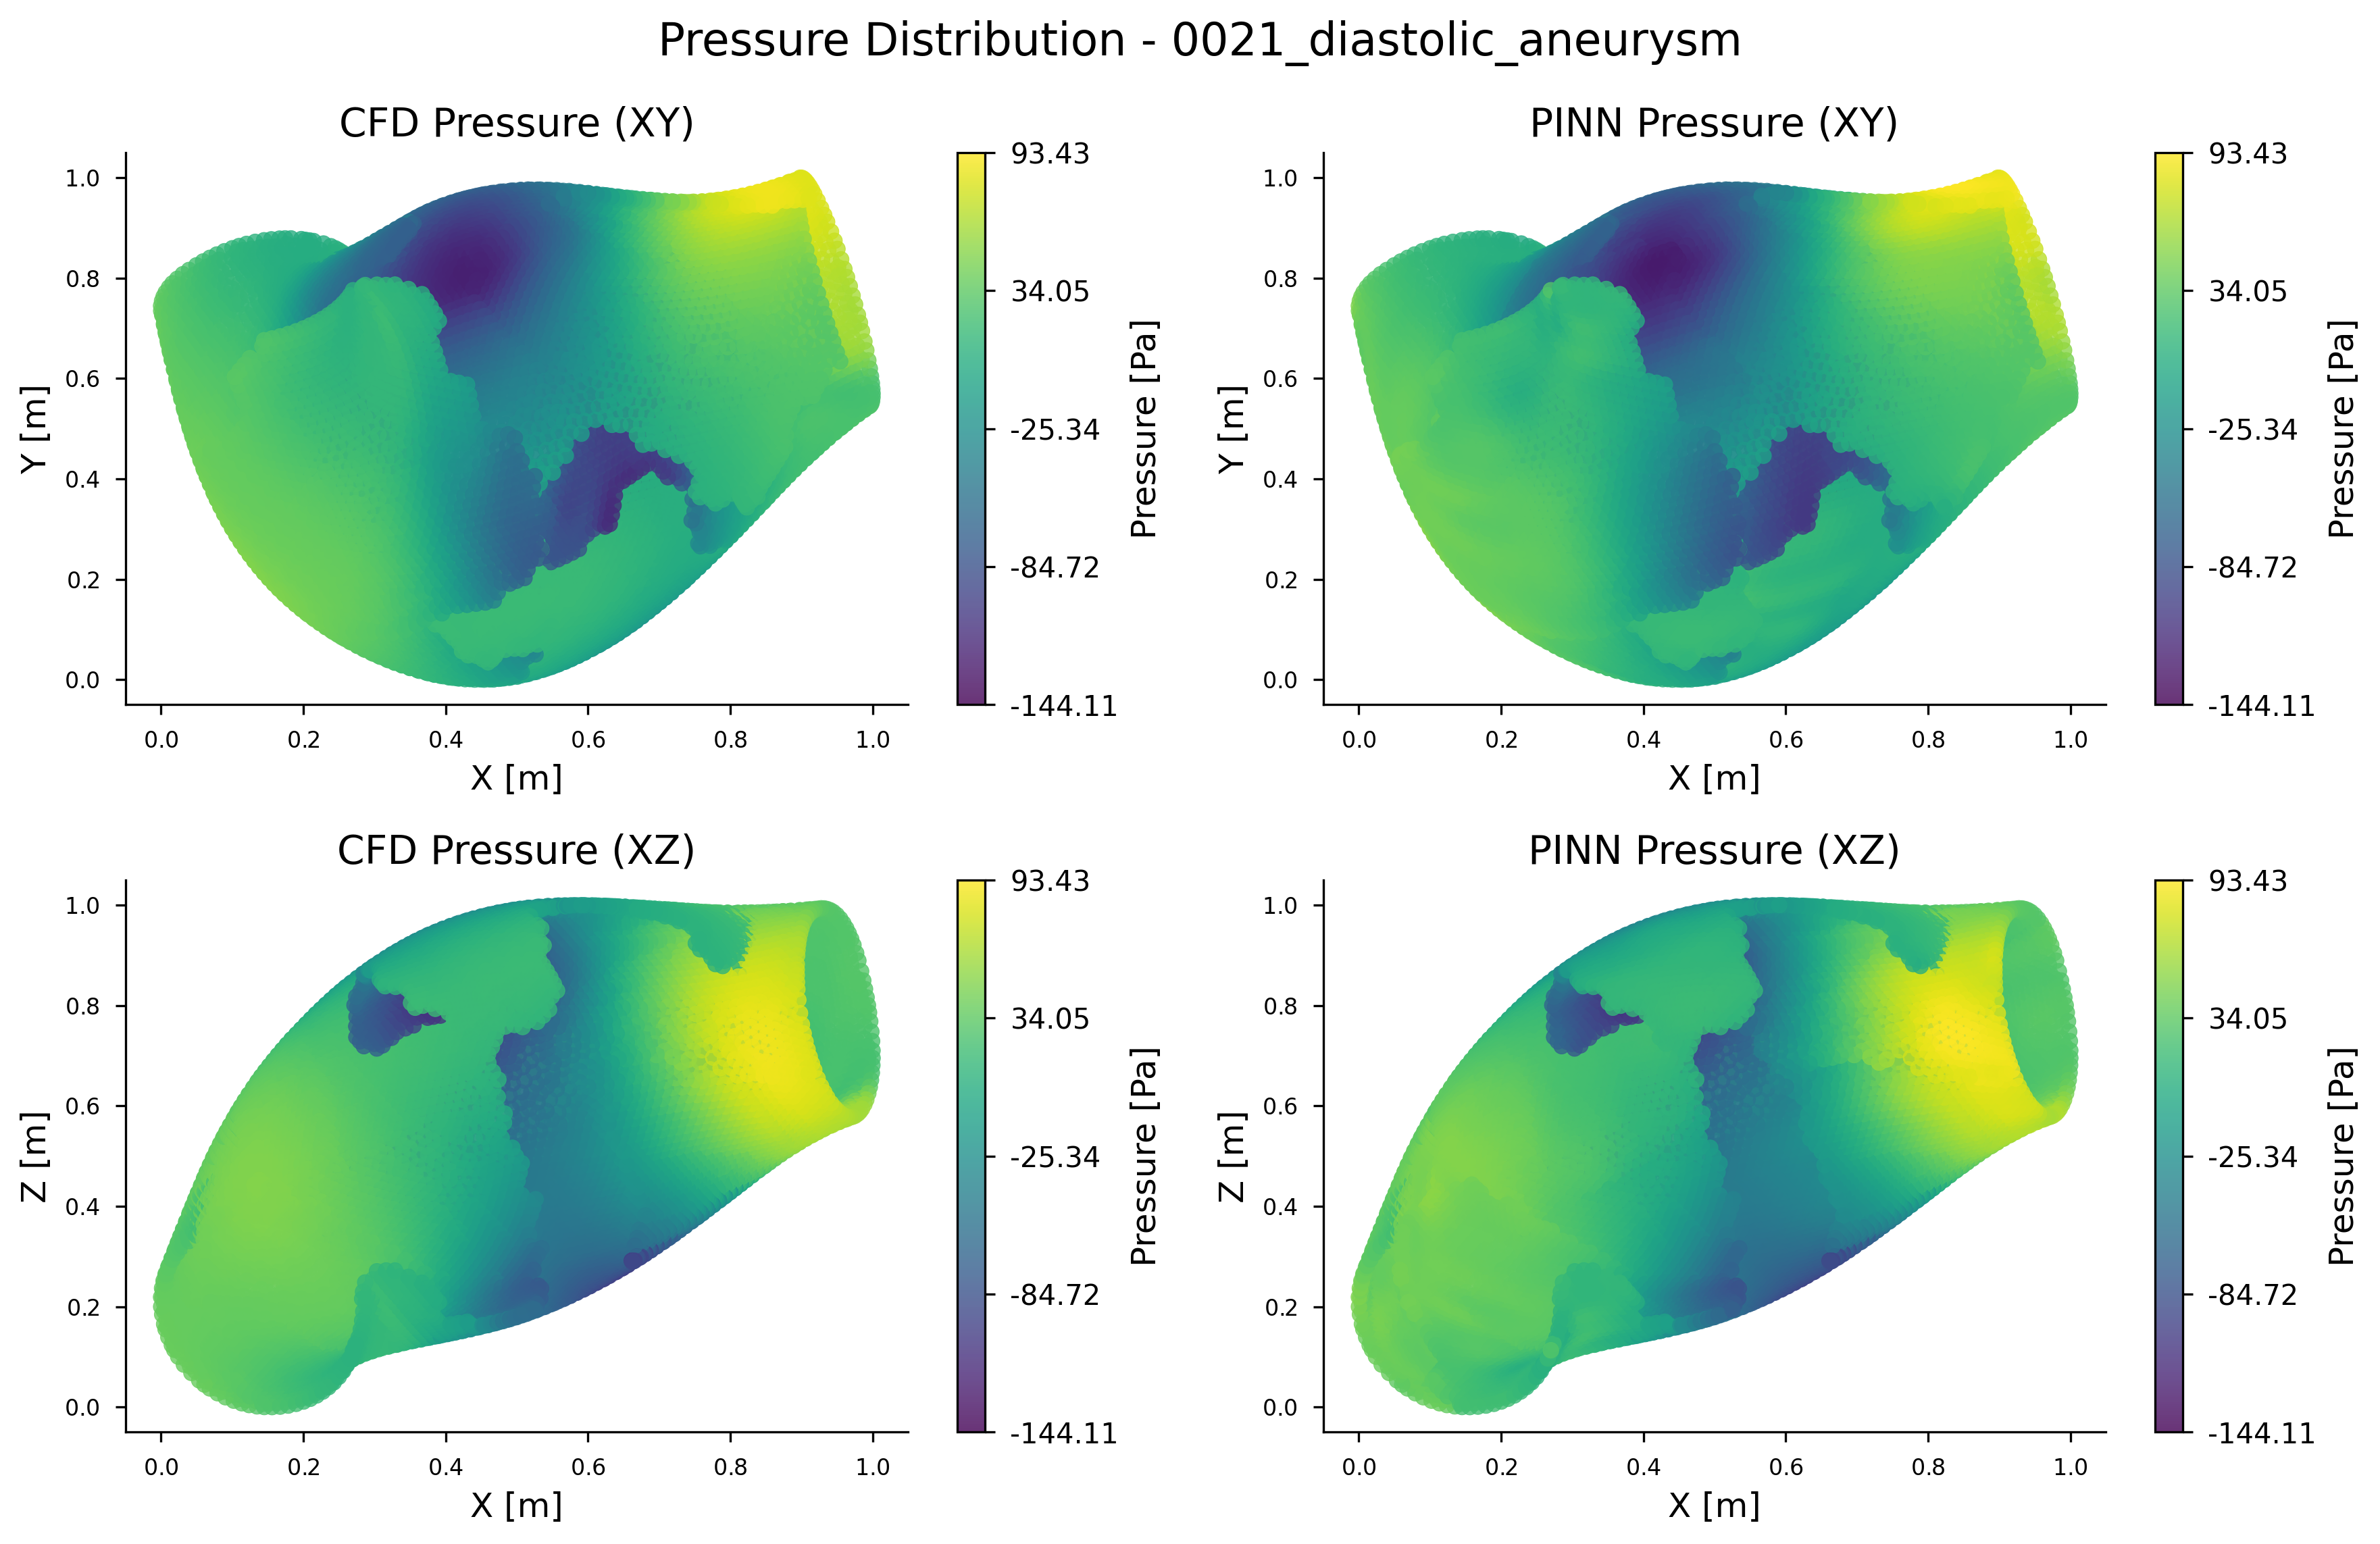
\includegraphics[width=\textwidth]{0021_diastolic_aneurysm/pressure_distribution_0021_diastolic_aneurysm.png}
        \caption{\small Pressure distribution}
    \end{subfigure}
    \begin{subfigure}{0.9\textwidth}
        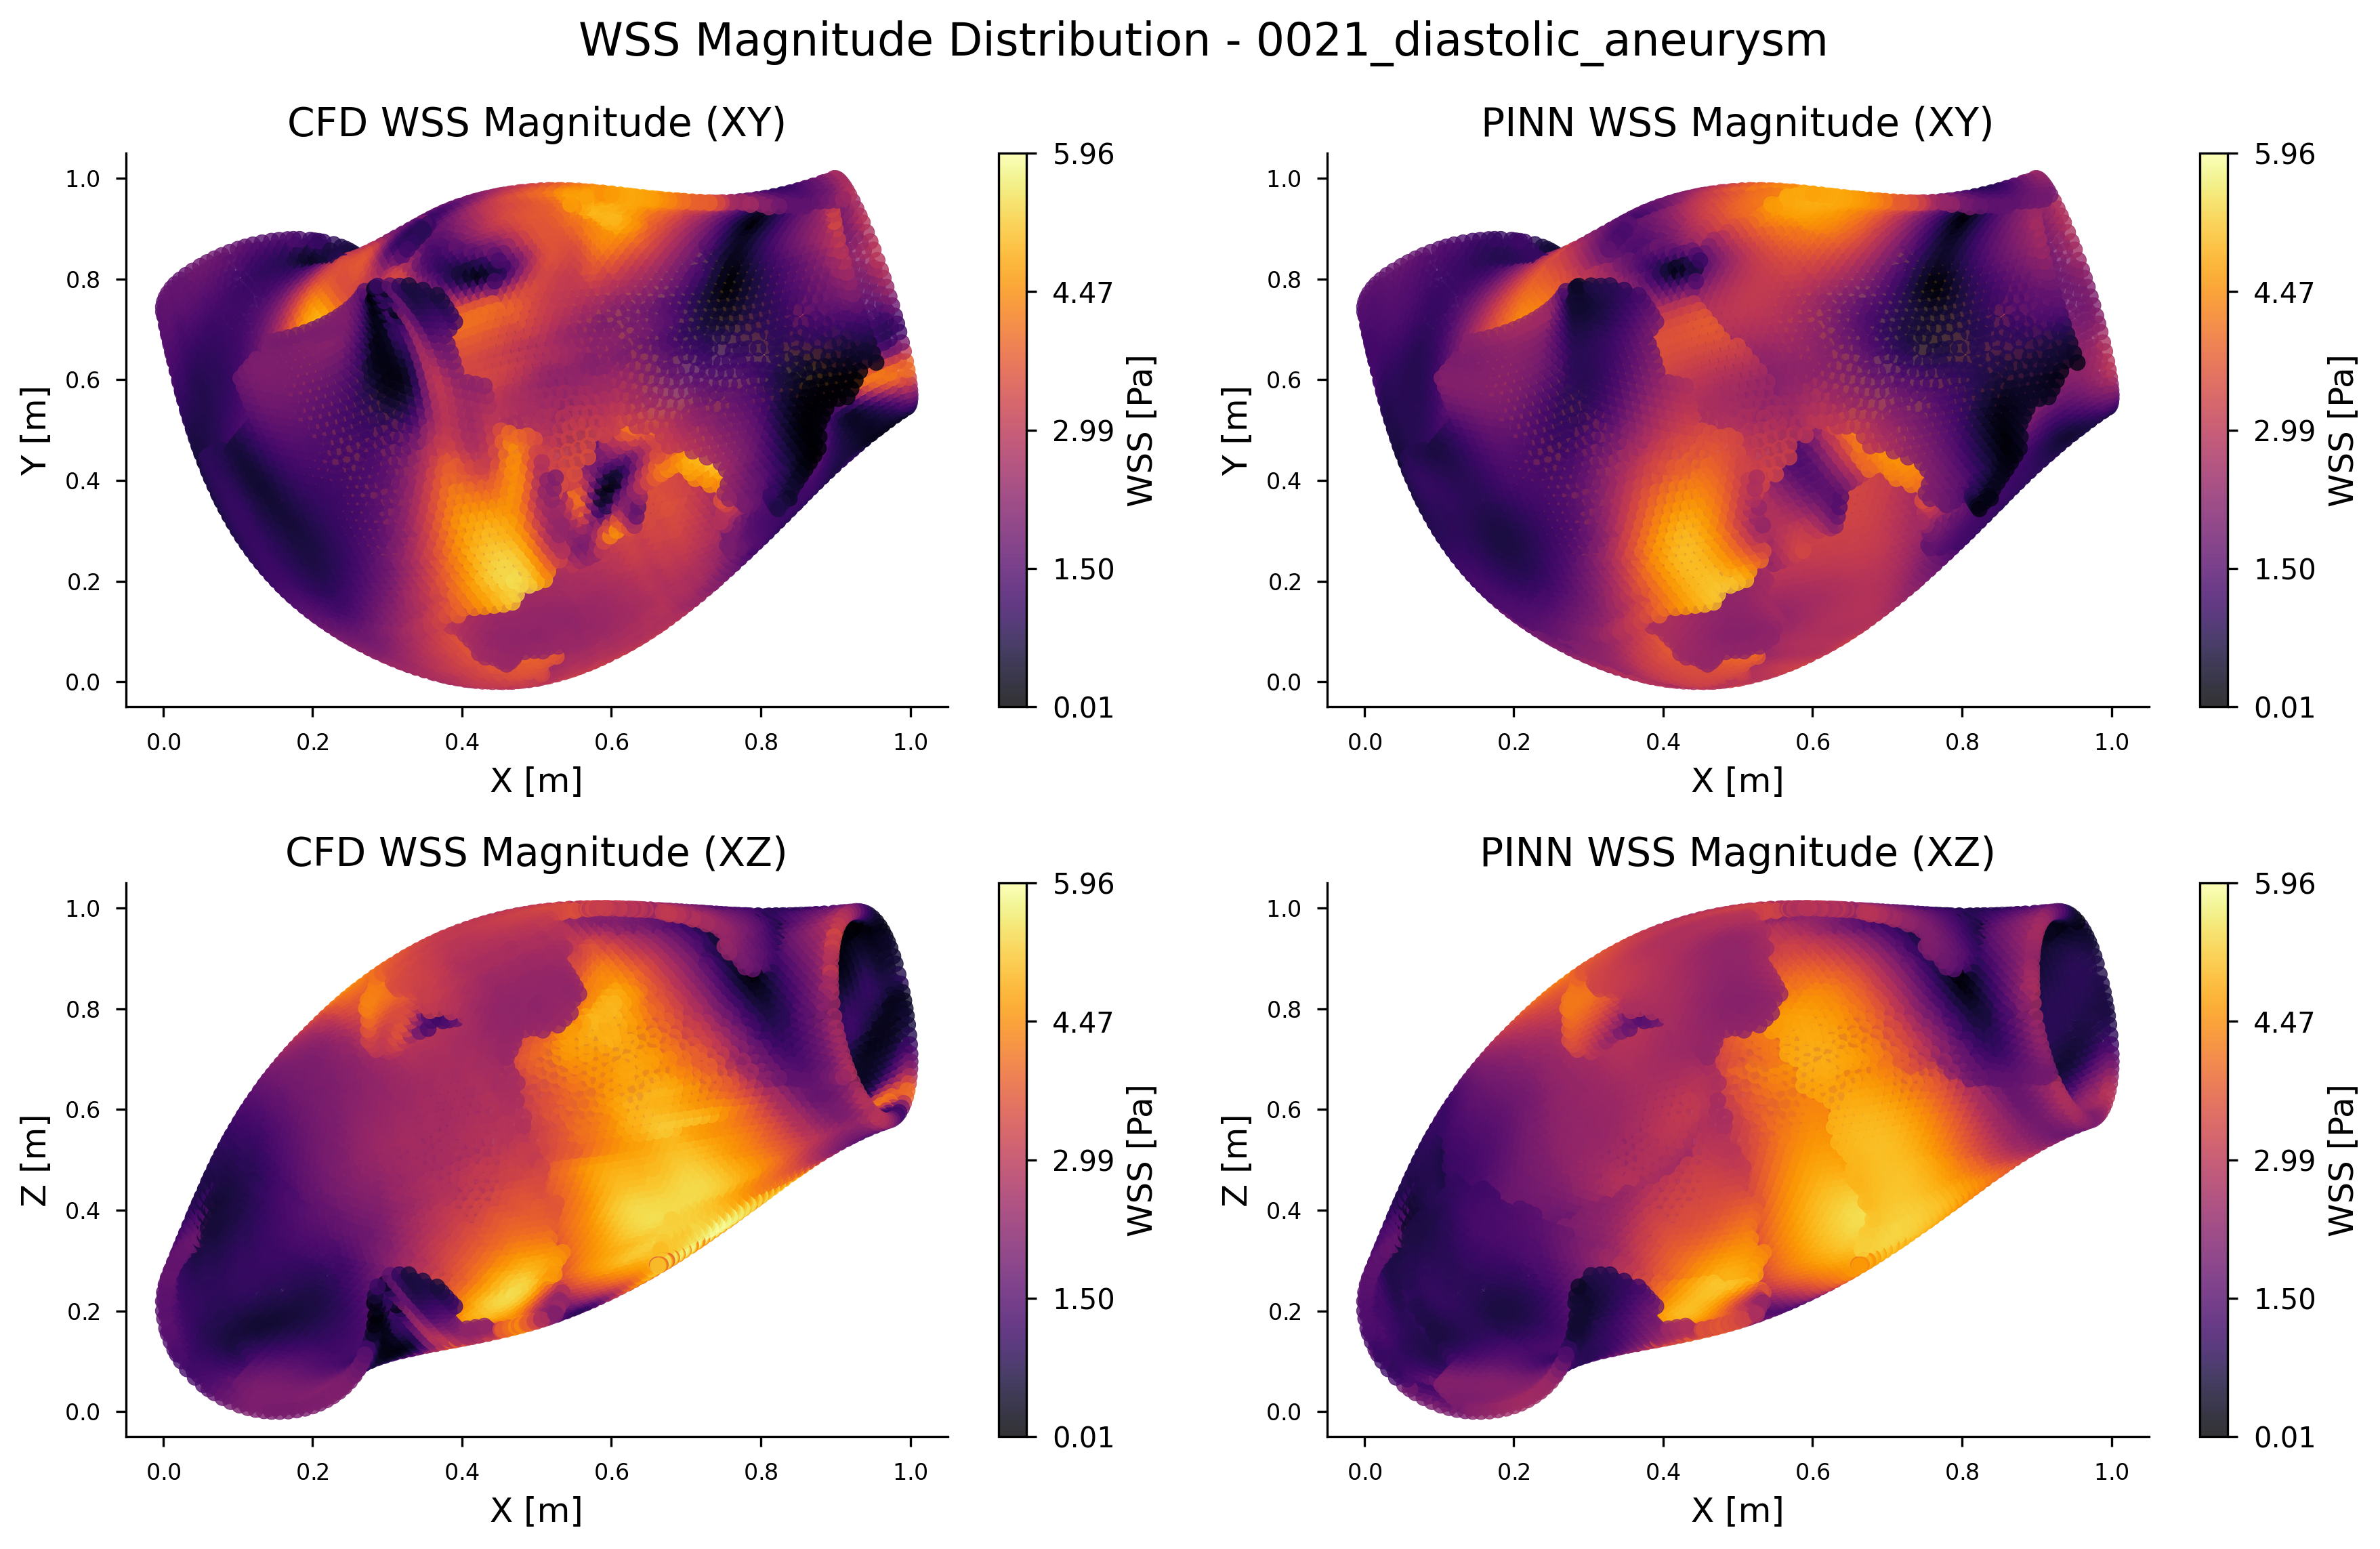
\includegraphics[width=\textwidth]{0021_diastolic_aneurysm/wss_magnitude_distribution_0021_diastolic_aneurysm.png}
        \caption{\small Wall shear stress}
    \end{subfigure}
    \caption{Von Mises stress (Pa) and wall shear stress contours for diseased cases. Figures a–d in each show the \(xy\) and \(xz\) planes for case 0021 dystolic aneurysm comparison between CFD and PINN results.}
    \label{fig:PINN_results1}
\end{figure}

\begin{figure}[H]
    \centering
    \scriptsize
    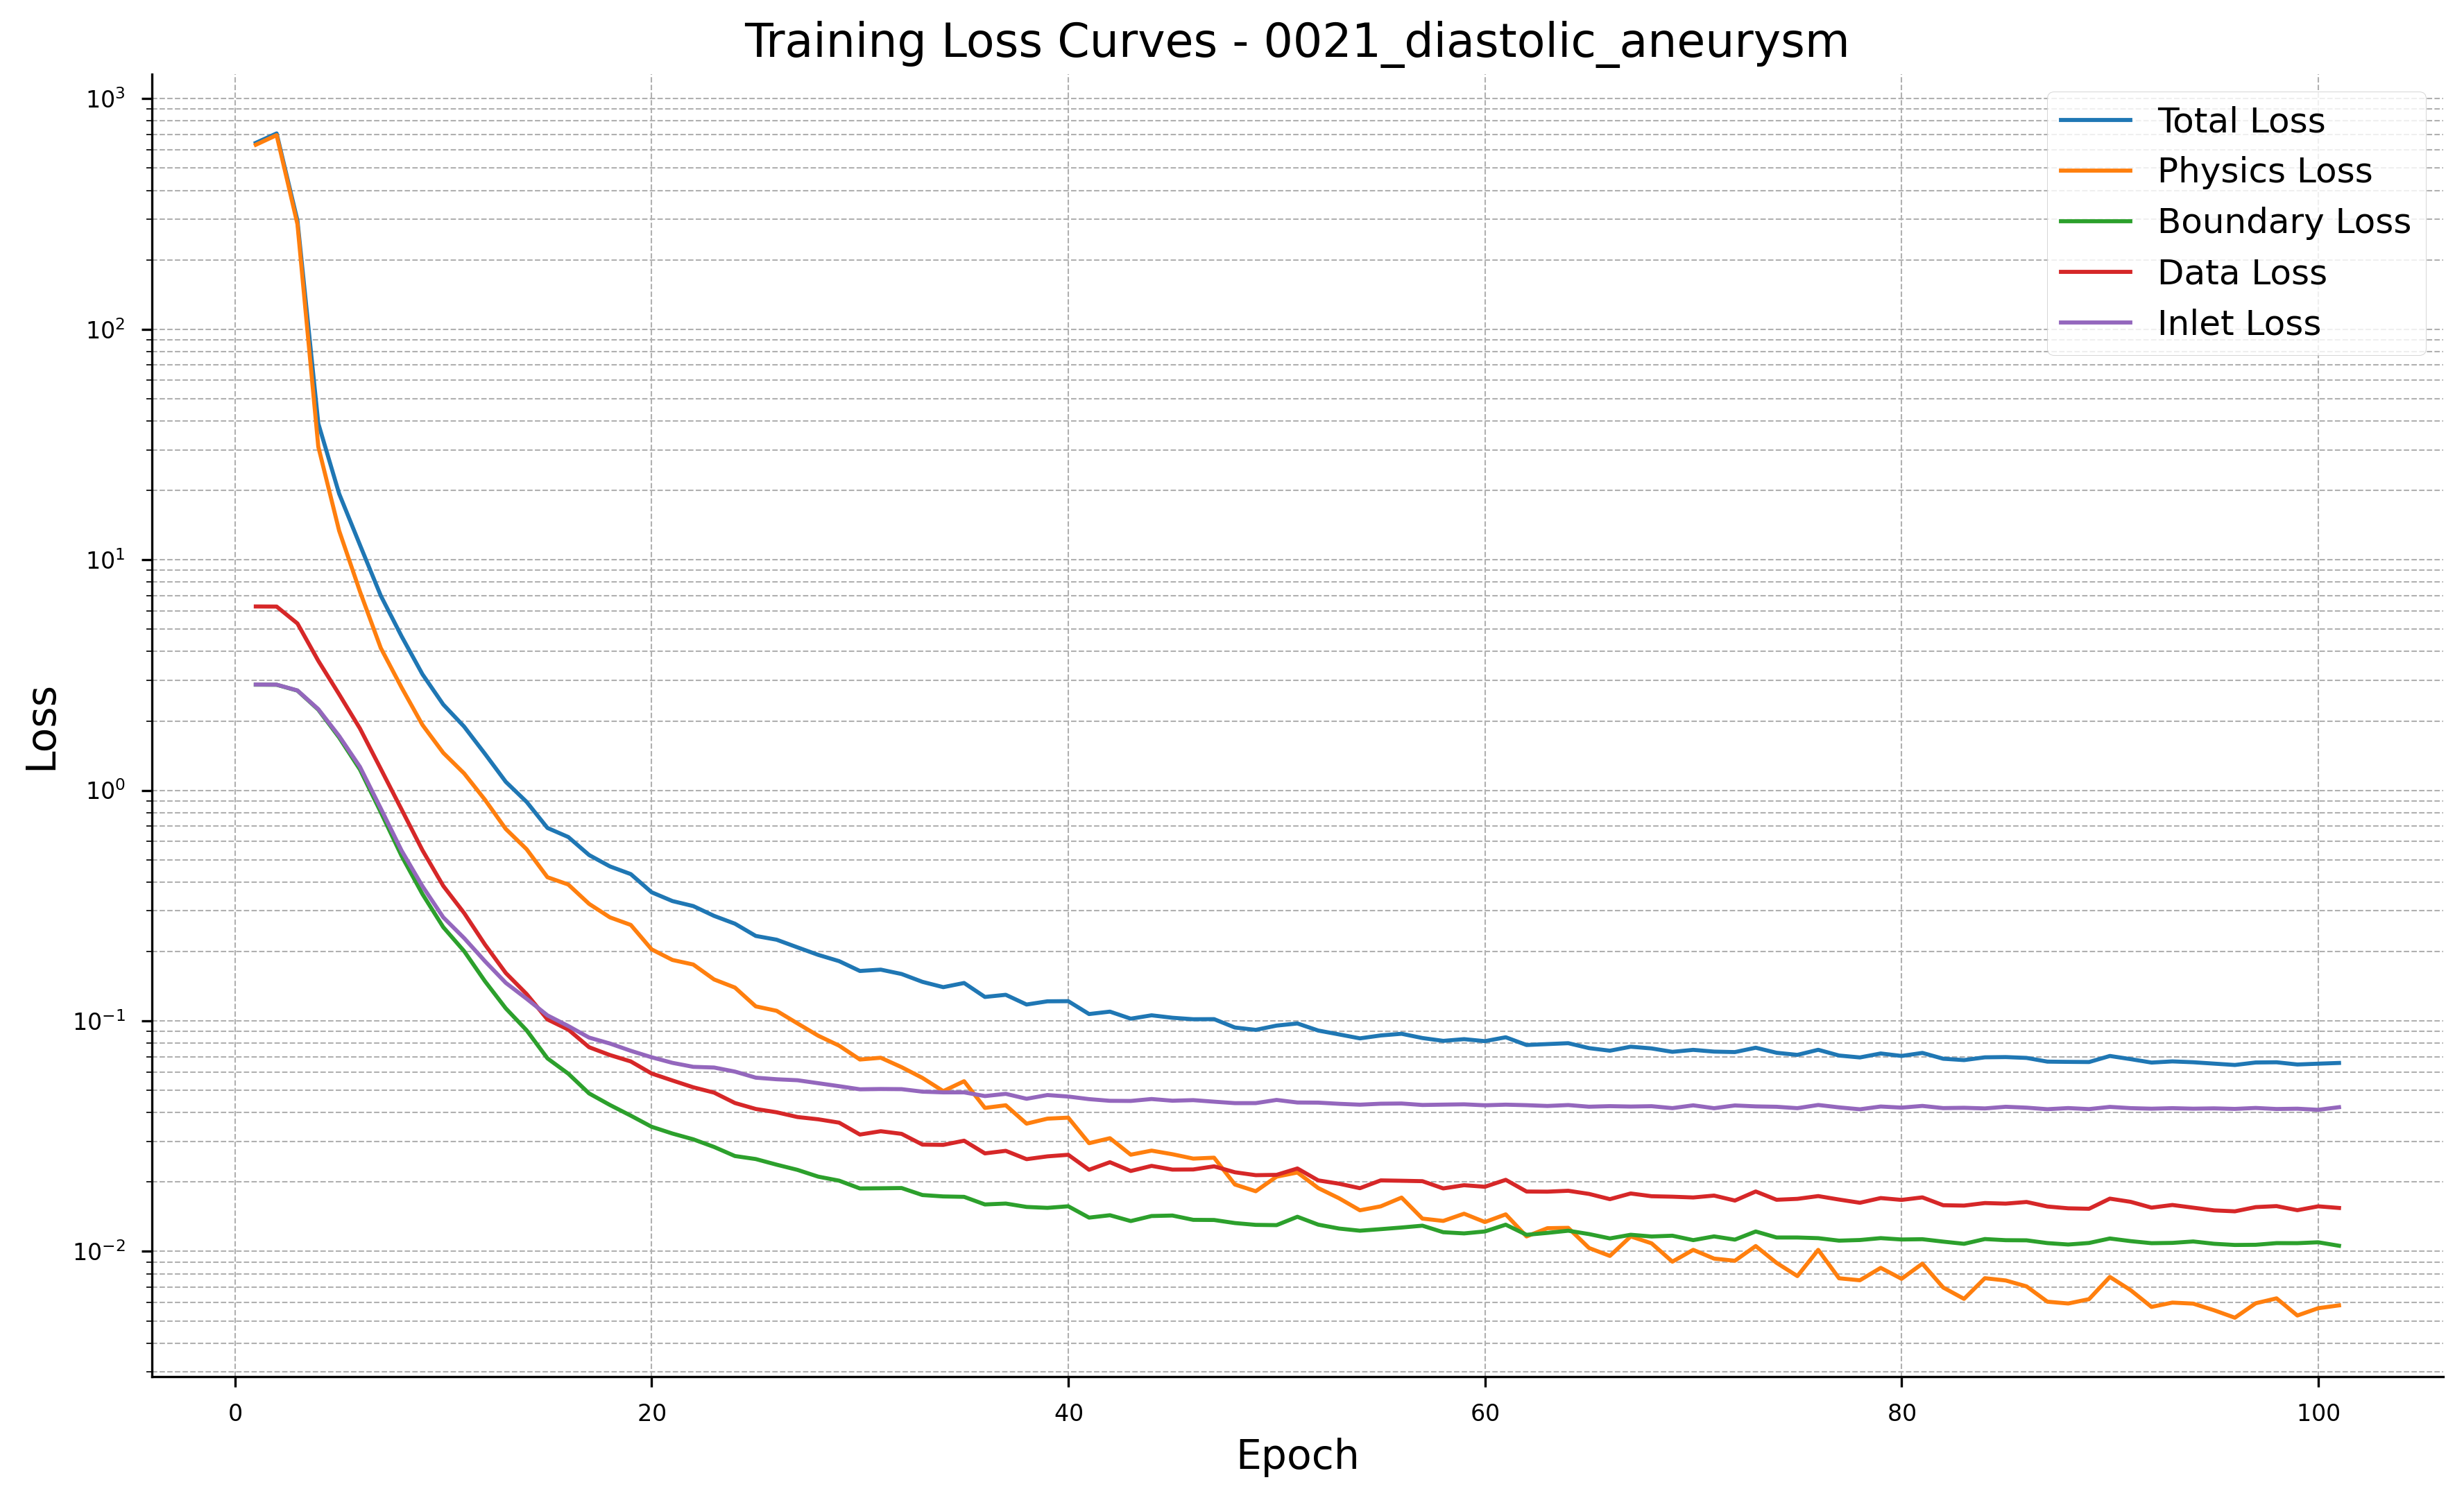
\includegraphics[width=0.9\textwidth]{0021_diastolic_aneurysm/0021_diastolic_aneurysm/loss_curves_0021_diastolic_aneurysm.png}
    \caption{Loss curves for the PINN training process, showing the evolution of the physics, boundary, inlet, and data-fitting losses over 1000 epochs. The self-adaptive loss weighting mechanism effectively balances the contributions of each loss component, ensuring that the network learns realistic flow solutions while adhering to the governing Navier--Stokes equations.}
    \label{fig:loss_curves1}
\end{figure}

Figure~\ref{fig:PINN_results1} illustrates the comparison between PINN predictions and CFD reference data for both pressure and WSS. The subfigures demonstrate the spatial distribution of pressure and WSS on both the \(xy\) and \(xz\) planes for a representative aneurysm case (0021 diastolic aneurysm). These visual comparisons confirm that the PINN accurately reproduces the key flow features observed in the CFD simulations. Furthermore, Figure~\ref{fig:loss_curves1} presents the evolution of the loss curves over 1000 training epochs, highlighting the convergence behavior of the physics, boundary, inlet, and data losses. The steady decline of these loss components reflects the efficacy of the self-adaptive weighting mechanism in guiding the network toward a physically consistent solution.

The mesh-free nature of PINNs \citep{raissi2019physics} enables the rapid evaluation of flow fields at arbitrary spatial and temporal resolutions, facilitating detailed hemodynamic analyses and personalized treatment planning. By leveraging the self-adaptive loss weighting scheme, the PINNs effectively balance the physics residuals, boundary conditions, and data-fitting objectives, ensuring that the network learns realistic flow solutions while adhering to the governing Navier--Stokes equations. The results presented here demonstrate the potential of PINNs as a powerful tool for simulating pulsatile flow in arterial geometries, with applications ranging from disease diagnosis to treatment planning and optimization.


\bibliographystyle{unsrtnat}
\bibliography{references}

\end{document}

